% CREATED BY DAVID FRISK, 2015
\chapter{Theoretical Framework}

\lettrine[findent=2pt]{\fbox{\textbf{T}}}{ }his chapter introduces theory that is related to this study covering the areas of architectures in automotive domain, the two types of electrical architectures at VCG, and the proprietary tool the Database that stores the low-level architecture. Basic knowledge of Model-Driven Software Engineering is presented, including the difference types of stakeholders. Related works are also discussed through out the chapter.

\section{Architectures in automotive domain}
Proper architecture is necessary for designing and building modern vehicles which are mostly driven by electronics and software. In this section, we have explained some related works of how an architecture plays an important role in automotive domain.\\

Beeck \cite{Beeck} developed a modeling approach for development of software for ECUs at BMW Group, which supports the development of logical and technical architectures (high- and low-level architectures, respectively). The approach was developed based on the notation Unified Modeling Language for Real-Time (UML-RT) aimed at compromising the complexity issue of developing, integrating, and maintaining software-intensive systems in vehicles. The logical architecture model was developed using UML-RT's capsule structure diagrams representing graphical system view of automotive functions. The technical architecture separated into software and hardware architectures was developed using UML-RT's component diagrams (for software) and deployment diagrams (for hardware). \\

For the logical architecture, the author created a UML-RT constructs and used them to model the architecture. From the meta-model (figure \ref{fig:beeck_metalmodel}), capsules, ports, protocols, signals, and connectors notations were used for modeling architectural artifacts. Capsules represent functions, while ports and protocols model function interfaces. A port was used to specify a communication point of a capsule. Each port had associated protocol, which contained two sets of signals: export and import. Connectors represented channels between function interfaces. \\

For the technical architectures, Components were used to model software components. Hardware components such as ECUs and sensors were modelled using UML-RT nodes. \\

The author also reported some problems regarding the use of UML-RT. One of the problems was, the set of UML-RT diagram notations was quite restricted. It was hard for ECU developers, who were familiar with non-object-oriented notations, to work with. In addition, the two protocols associated with ports did not meet requirements of some ECUs.

\begin{figure}[H]
\centering
\captionsetup{justification=centering}
\vspace{0cm}% Adjust vertical spacing here
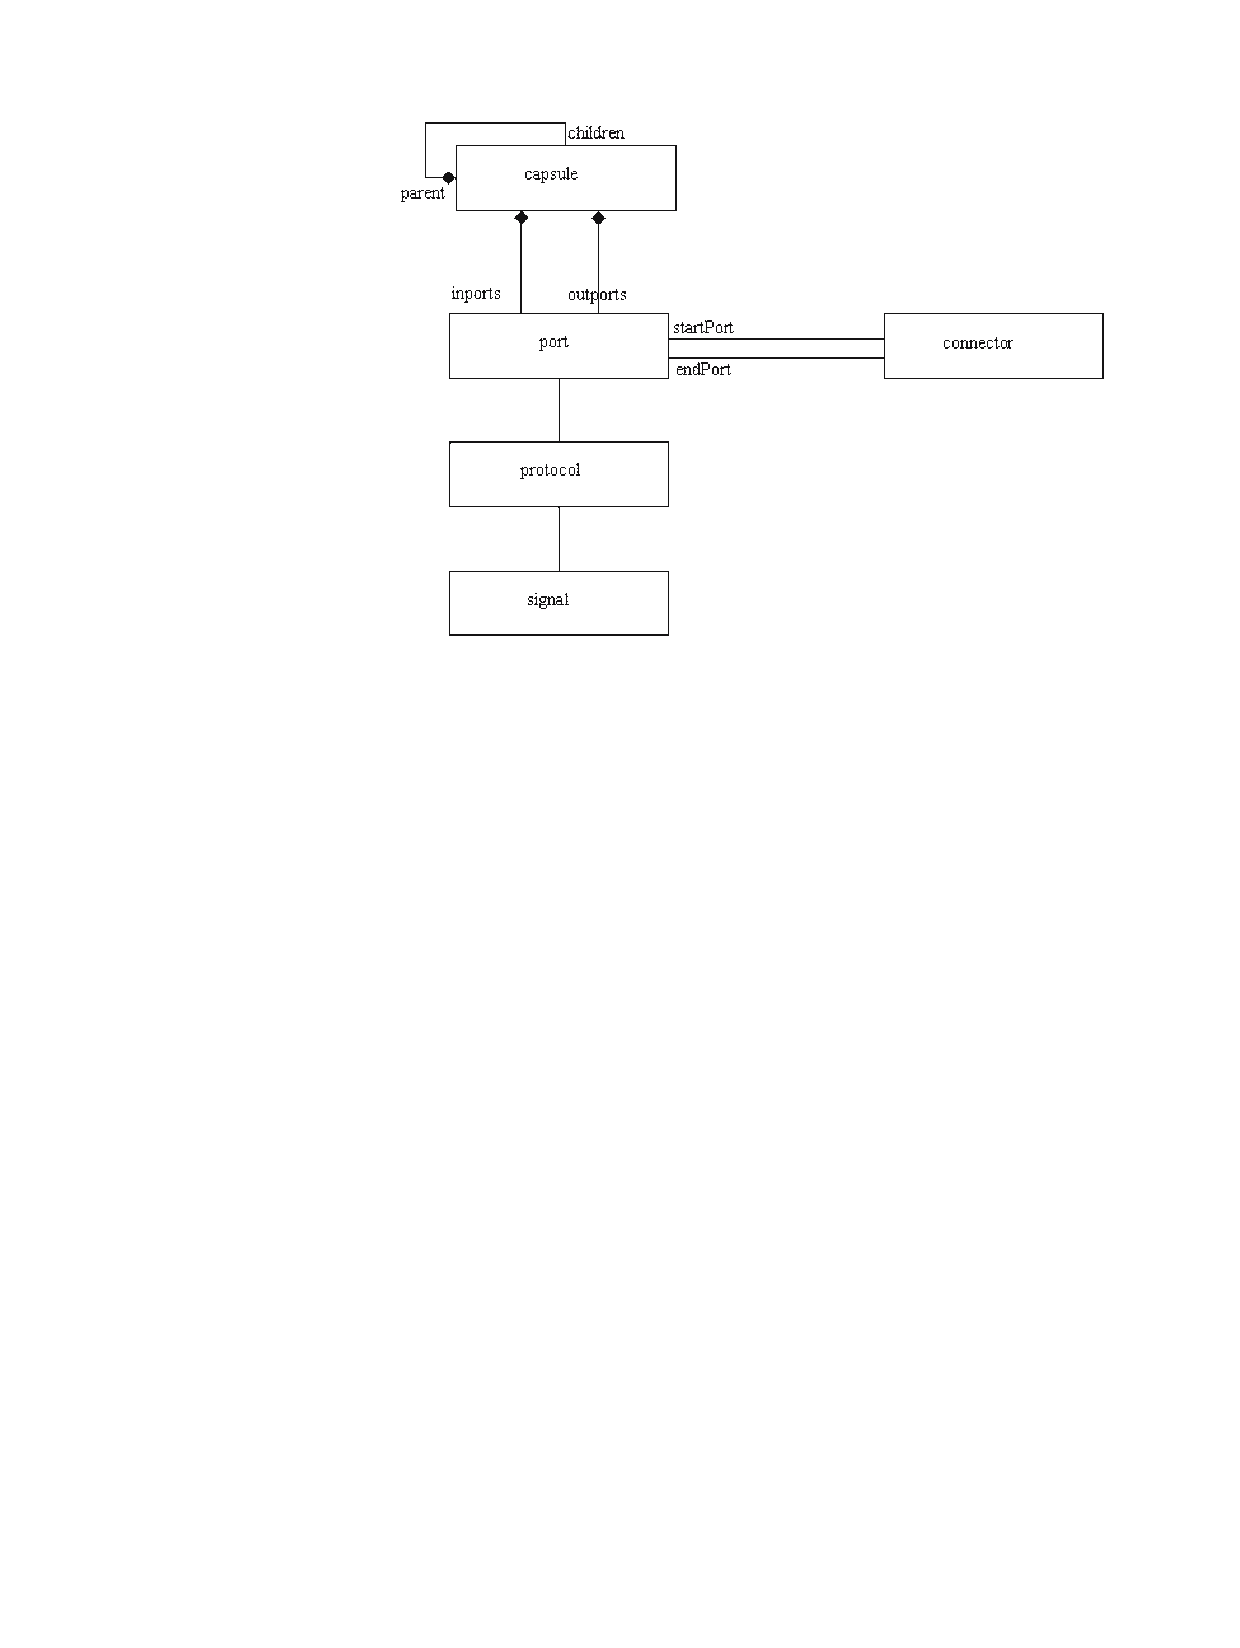
\includegraphics[width=0.55\linewidth]{figure/literatures/beeck_metalmodel.pdf}
\caption{Meta-model of UML-RT constructs for logical architecture \cite{Beeck}}
\label{fig:beeck_metalmodel}
\end{figure}

Grönniger et al. \cite{Grönniger} developed an approach for modelling logical architectures of automotive systems using views. Function nets which are valid Systems Modeling Language (SysML) Internal Block Diagrams (IBD) were used to model complete automotive functions and views which described the environment and context of a certain aspect of function net. In addition to that, views could be used to model features in a self-contained way, and to specify consistency conditions for consistency between a view and a function net.\\

The authors claim that function nets and views could be used to describe and to explain scenarios of use-cases like how an automotive system reacts to external events or failures caused by subsystems. However, numerous models had to be created as well as references between these models. The authors states in their work that an investigation of existing model management strategies to handle number of models would be performed in the future.\\

Dajsuren \cite{Dajsuren} presented a research which was part of Hybrid innovations of Trucks and it covers the automotive Architecture Description Language (ADL) and quality of automotive software. This research had a role of identifying a proper ways of developing automotive software. \\

The author suggests that automotive software development enabled interaction between different engineering fields such as mechanical engineering, electrical engineering and software engineering. ADL was said to be an effective way to manage such multi-disciplinary engineering information. It had been defined on this paper as ``one of the approach to formalize the representation of the automotive systems and software architecture''. Examples of ADL used in automotive companies are definition of AML for BMW company, EAST-ADL and TADL for Volvo, Fiat, and VW/Carmeq. \\

The different levels of the architecture had been mentioned as well, these include:
\begin{itemize}
    \item \textit{Feature view} that shows number of features in a system.
    \item \textit{Function view} that shows a number of functions or subsystems in a system. A single feature could include one or more function.
    \item \textit{Software view} that shows a detailed architecture. It shows components and blocks which represent the implementation of the functions specified in the function view.
    \item \textit{Hardware view} that contains ECUs, sensors, actuators and Controller Area Network (CAN).
\end{itemize}
\vspace{0.2cm}
The author decided to use ADL language SysML\footnote{\url{https://sysml.org}} in modelling a functional architecture (view) and MATLAB/Simulink had also been mentioned as one of the most popular graphical modelling language and a simulation tool for modelling software architecture (view). \\

The inconsistency of architecture in multiple views had also been explained. This is one of the problem that VCG also experiences which is in between the high- and low-level architectures. In this paper, a consistency rule had been proposed between the different views of the architecture.

\subsection{Low- and high-level electrical architectures at VCG}
To have a better understanding of how low- and high-level electrical architectures have been constructed and used in VCG. We studied some related works that were conducted in the company.\\

Eliasson et al.~\cite{Eliasson_1} found that VCG and Volvo Group Truck Technology (VGTT) have two types of architecture: a high-level architecture and a working architecture (low-level architecture). The high-level architectures produced by high-level architects contain design decision, principles, rules, and pattern that should govern the overall system. The working architecture produced by low-level architects contains logical components which are broken down from the high-level architecture and more details. The study shows that the working architecture is always kept updated by developers as the product evolve, while the high-level architecture is only updated when the project has started. Because of this reason, the inconsistency between the two architecture occurs. They also suggest that having two different groups of architects result to problems. High-level architects have a thought that the low-level architects are very focused on short-term solutions which makes them miss an overall picture of the system, while low-level architects see that another group lacks an understanding of current situation and is too focused on solutions that might be good in long run. \\

In another related work, Eliasson et al. \cite{Eliasson_2} also suggest that the presence of the Architecture Technical Debt (ATD) at the design level at VCG plays an important role on the efficiency of communication between components. In this paper, there is a discovery of the ATD items (architectural violations) such as the misplaced LCs and their impacts on the software development process (see figure \ref{fig:eliasson_atd}). The ATD items together with the inputs from the stakeholders at VCG were used to assist in creating a visual tool which provides a better visualization of the ATD items and its interest. With this tool, the visualization is more comprehensive to the stakeholders. 

%FIGURE
\begin{figure}[H]
\centering
\captionsetup{justification=centering}
\vspace{0cm}% Adjust vertical spacing here
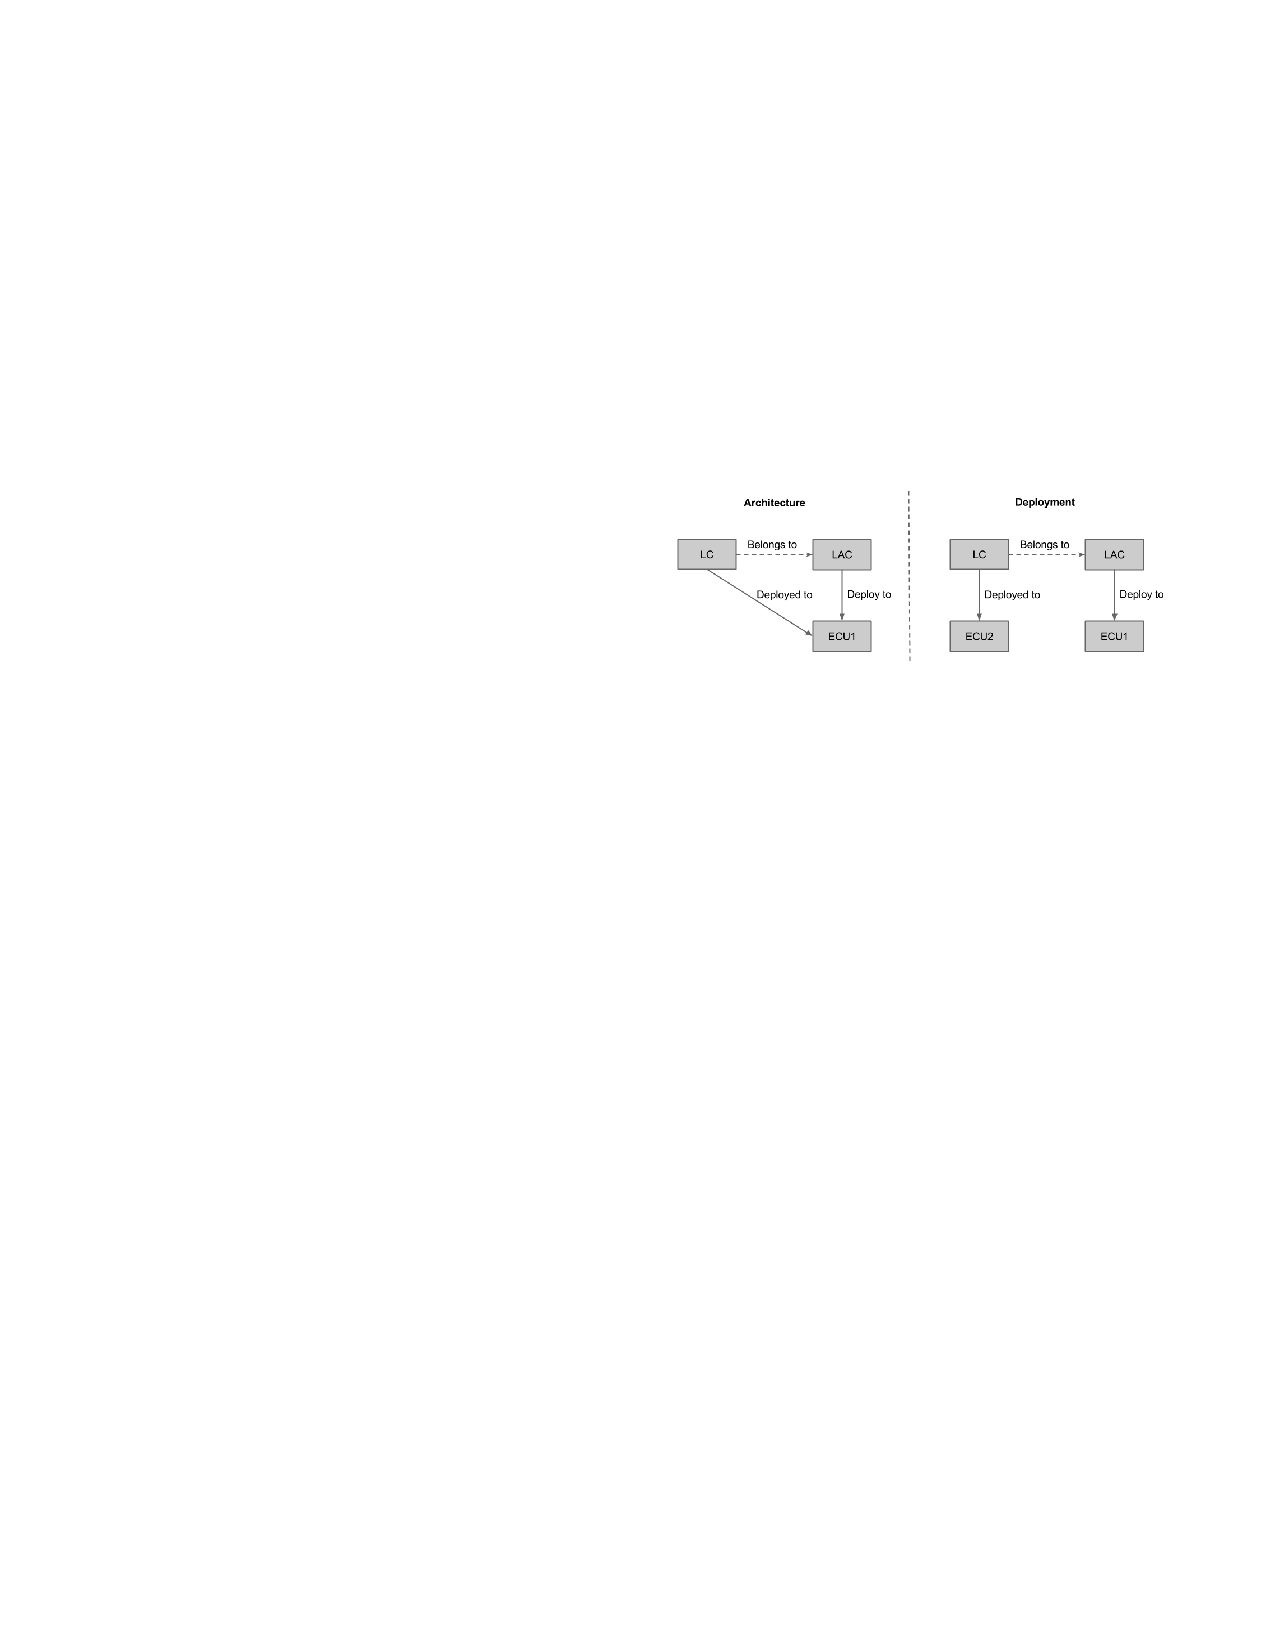
\includegraphics[width=0.7\linewidth]{figure/literatures/eliasson_atd.pdf}
\caption{The difference between architectural design and actual deployment \cite{Eliasson_2}, \copyright2015 IEEE}
\label{fig:eliasson_atd}
\end{figure}

%%%
\section{Software visualization}
The emerging of component based software are said to have a repercussions on software visualization. On visualizing a component-based software product, one has to consider a visualization of  component model, software components and of software assemblies. Favre and Cervantes~\cite{Jean} suggest to visualize a component model by describing it as a set of UML class diagram (meta-model). The meta-model will have all the necessary concepts to describe components without getting to the implementation details. The concept of meta-modelling can be considered as a basis in specifying a graphical notation of visualizing components. The graphical notation simplifies the understanding of a meta-model. On visualizing components, a specific notation must be used for each component technology. The authors also mentioned the usefulness of a graphical notation that it allows software engineers to communicate without the burden of speaking in technical terms.\\

Most software engineers think in low-level programming when designing a component model rather than a conceptual entities. Favre and Cervantes mentioned the useful of having the visualization of the software products to software engineers since they designed the model `blindly', so the visualization would help them to get a complete overview of the implementation. They also elaborated several options that we could apply in visualizing the data stored in the Database. Some challenges had been mentioned in visualizing complex components which might have many ports, so in this case, hiding ports with no connection and show only ports with connection could be of useful when it comes to a visualization process. Another challenge that was mentioned was the visualizing the components with complex connectors.\\

The visualization was also done at in Ericsson, where the task was to recover the architecture, it involved getting models from a source code. Darvas and Konnerth~\cite{Adam} mentioned on the advantages of having an automated visualization as it makes the architecture consistent with the current implementation found in a source code. In their work, they mentioned on grouping the ports using cable and port group pattern, it was the technique to merge the connectors to a single connector. The use of abstraction pattern could be useful in our case as the single component can have many ports and hence make the diagram not readable. In our case, we may be needed to find the corresponding metrics that will help to group the ports based on some similarities. Another thing that was mentioned in the work was the way of preserving the hidden information, this implies that once the artifacts are grouped, there will not be a way to see what is inside the grouped artifacts so instead, a comment (text) next to the grouped artifacts can be useful to briefly describe what is inside of it.


\section{Model-Driven Software Engineering}
In creating a visualization of the electrical architectures, we applied Model-Driven Software Engineering methodology to our work. This section aims at giving the readers basic knowledge of the method.\\ 

In software development, models are used to depict software artifacts in software engineering activities throughout software development life cycle. A model itself is used as primary artifact representing more abstract view of a software to be built. In this context, the methodology is known as \textit{Model-Driven Software Engineering} (MDSE), aiming at tackling the complexity problem caused by the large size of a software due to the needs of humans \cite{Brambilla}. The goals of MDSE also include increasing the software development speed which can be done by transformations (Chapter~\ref{model_transformation}), reducing cost in long-term, and supporting the reuse of model for repeatable processes. \\

Based on the book \textit{`Allgemeine Modelltheorie (General Model Theory)'} written by Stachowiak~\cite{Stachowiak}\footnote{ \url{https://modelpractice.wordpress.com/2012/07/04/model-stachowiak/} (english translation)}. He describes that a model should have 3 fundamental properties: \textit{reduction}, \textit{mapping}, and \textit{pragmatic}. Reduction property of a model is that it contains only details relevant to model creators and users. Generally speaking, the model does not include all details of its original. The mapping property means a model is always the model of something else i.e. its original. The pragmatic property of a model is the model can replace its original with respect to some purpose.\\

The core concept of MDSE can be explained in terms of equation based on the famous Wirth equation\footnote{For further discussion, see Wirth, N. (1976). \textit{Algorithms + data structures=programs}. Englewood Cliffs, N.J.: Prentice-Hall.}, as follows: 

\begin{equation}
Models + Transformations = Software
\label{eg:mde}
\end{equation}

\subsection{Modeling languages}
\label{sec:modeling_languages}
Models and transformations need to be defined in some notation which in MDSE context it is called \textit{modeling languages}. A modeling language is a tool that designers use for specifying definition of the concrete representation of a model for a software system \cite{Brambilla}. It is comprised of three main ingredients: \textit{abstract syntax}, \textit{concrete syntax}, and \textit{semantics} (see figure~\ref{fig:brambilla-modeling}). \\

\begin{figure}[H]
\centering
\captionsetup{justification=centering}
\vspace{0cm}% Adjust vertical spacing here
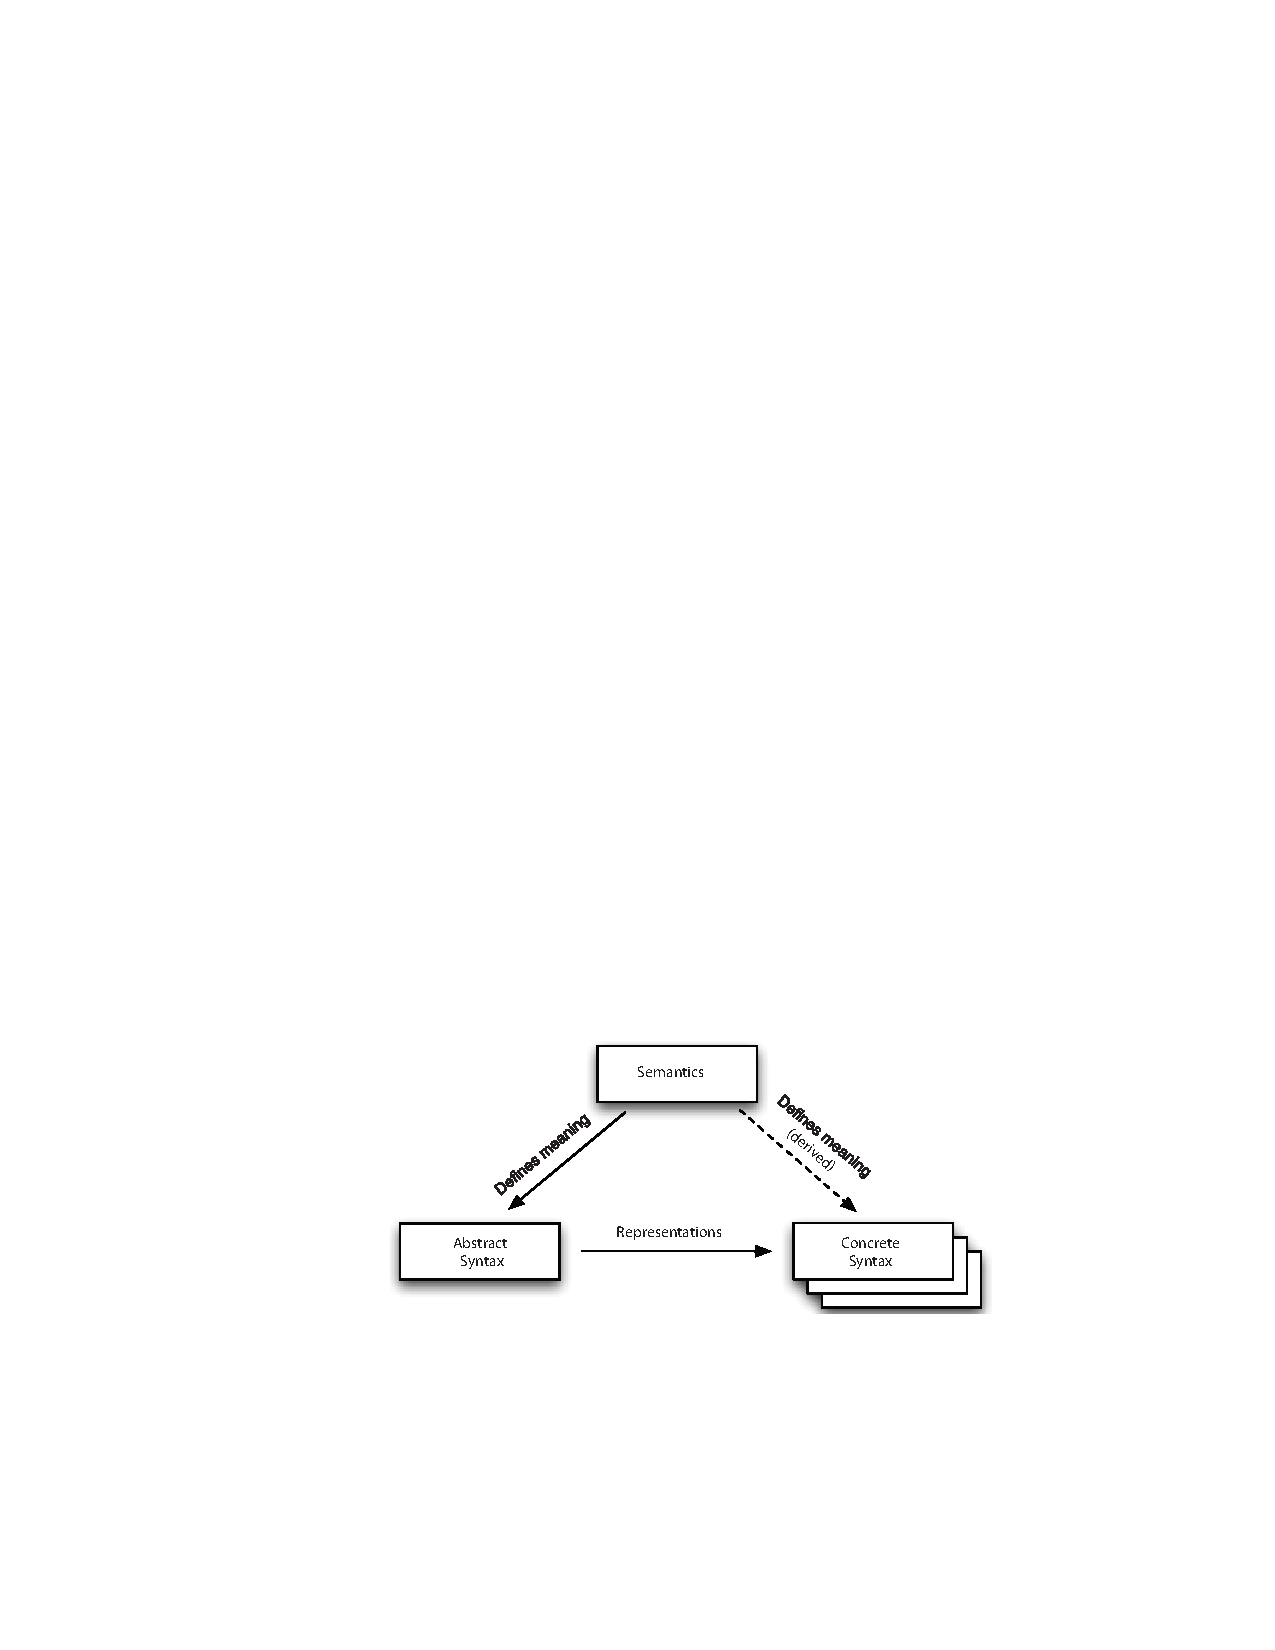
\includegraphics[width=0.6\linewidth]{figure/literatures/brambilla_modeling.pdf}
\caption{Three main ingredients that comprise a modeling language \cite{Brambilla}}
\label{fig:brambilla-modeling}
\end{figure}

A modeling language may consist of graphical representations, textual representations, or both. Modeling languages can be classified into two main categories: Domain-Specific Language (DSL) and General-Purpose Modeling Language (GPML, GML, or GPL). DSLs are the languages that are designed for specific domain, context, or company. The purpose of this type of languages is to help people to describe and explain things in a certain domain. In contrast, GPLs are the languages that are designed for general use. They lack specific features for a specific domain. An example of this type of languages is UML. \\

\subsubsection{Meta-models, model instances, and semantics}
As introduced in Section~\ref{sec:modeling_languages}, a modeling language is comprised of abstract syntax, concrete syntax, and semantics (see figure~\ref{fig:brambilla-modeling}). An abstract syntax is defined using \textit{meta-models} \cite{Brambilla}. A meta-model is a precise definition of the parts and rules needed to create valid models \cite{Tichy}, so to speak a type of model used to describe the model.\\

A concrete syntax is the concrete notation of a modeling language. It can be either a graphical or textual representation of \textit{model instances}. The figure~\ref{fig:brambilla-abstract-concrete} shows the abstract syntax and graphical concrete syntax of one of the well-known DSLs, simple Web Modeling Language (sWML). \\

The third ingredient of a modeling language is semantics. They define the meaning of abstract syntax and concrete syntax (indirectly). In software engineering, semantics are classified into two main categories: \textit{static semantics} and \textit{dynamic semantics}. The former specifies the allowed structure in a modeling language such as well-formedness and typing of meta-models, while the latter describes the execution behavior or run-time effect of a model \cite{Stuurman}.

\begin{figure}[H]
\centering
\captionsetup{justification=centering}
\vspace{0cm}% Adjust vertical spacing here
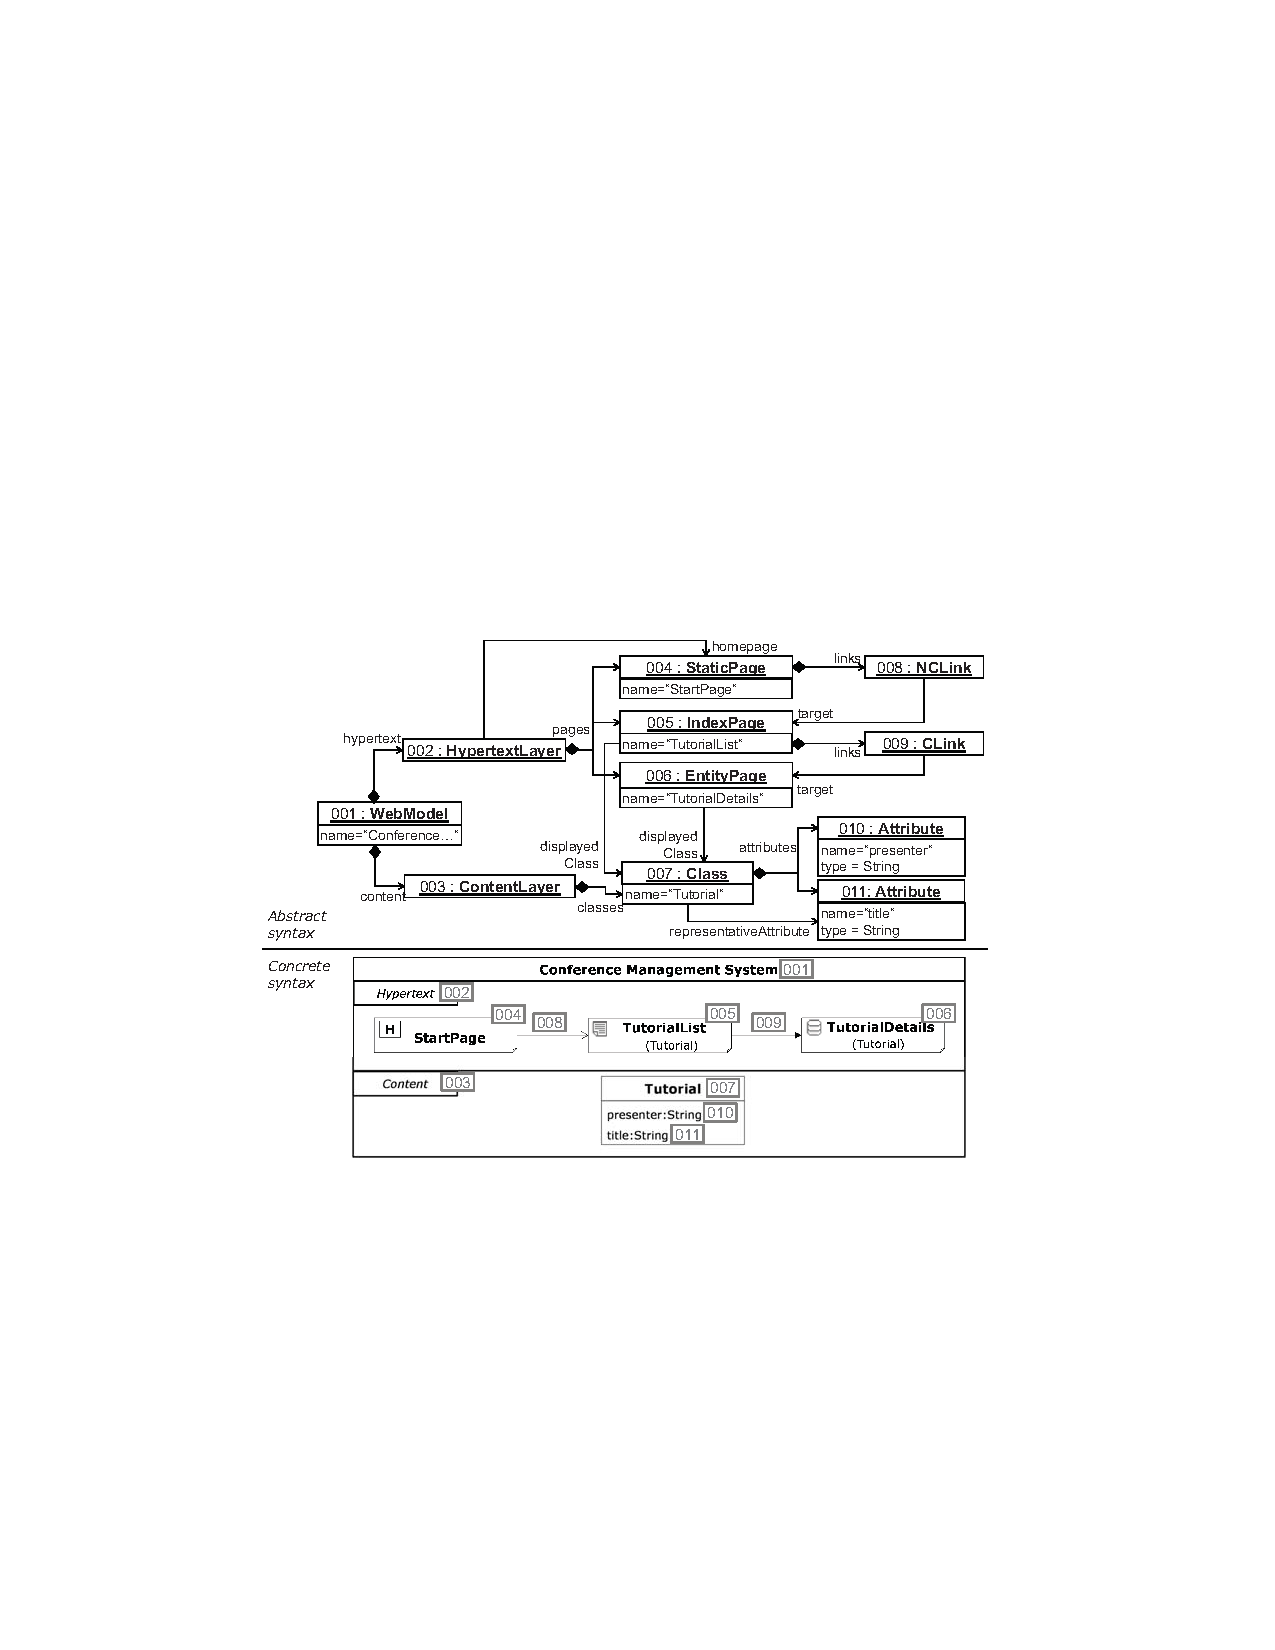
\includegraphics[width=0.75\linewidth]{figure/literatures/brambilla_abstract_concrete.pdf}
\caption{sWML model's abstract syntax and graphical concrete syntax \cite{Brambilla}}
\label{fig:brambilla-abstract-concrete}
\end{figure}

In an integrated development environment (IDE), such as Eclipse\footnote{\url{https://eclipse.org/}}, you can create a meta-model and a model instance by using Eclipse Modeling Framework (EMF) with an Eclipse plug-in called \textit{EcoreTools}\footnote{\url{http://www.eclipse.org/ecoretools/}}. EcoreTools is a complete environment including a Graphical Ecore Editor (Figure~\ref{fig:screenshot_ecore_editor}) for creating meta-models (Ecore) and model instances. 

\begin{figure}[H]
\centering
\captionsetup{justification=centering}
\vspace{0cm}% Adjust vertical spacing here
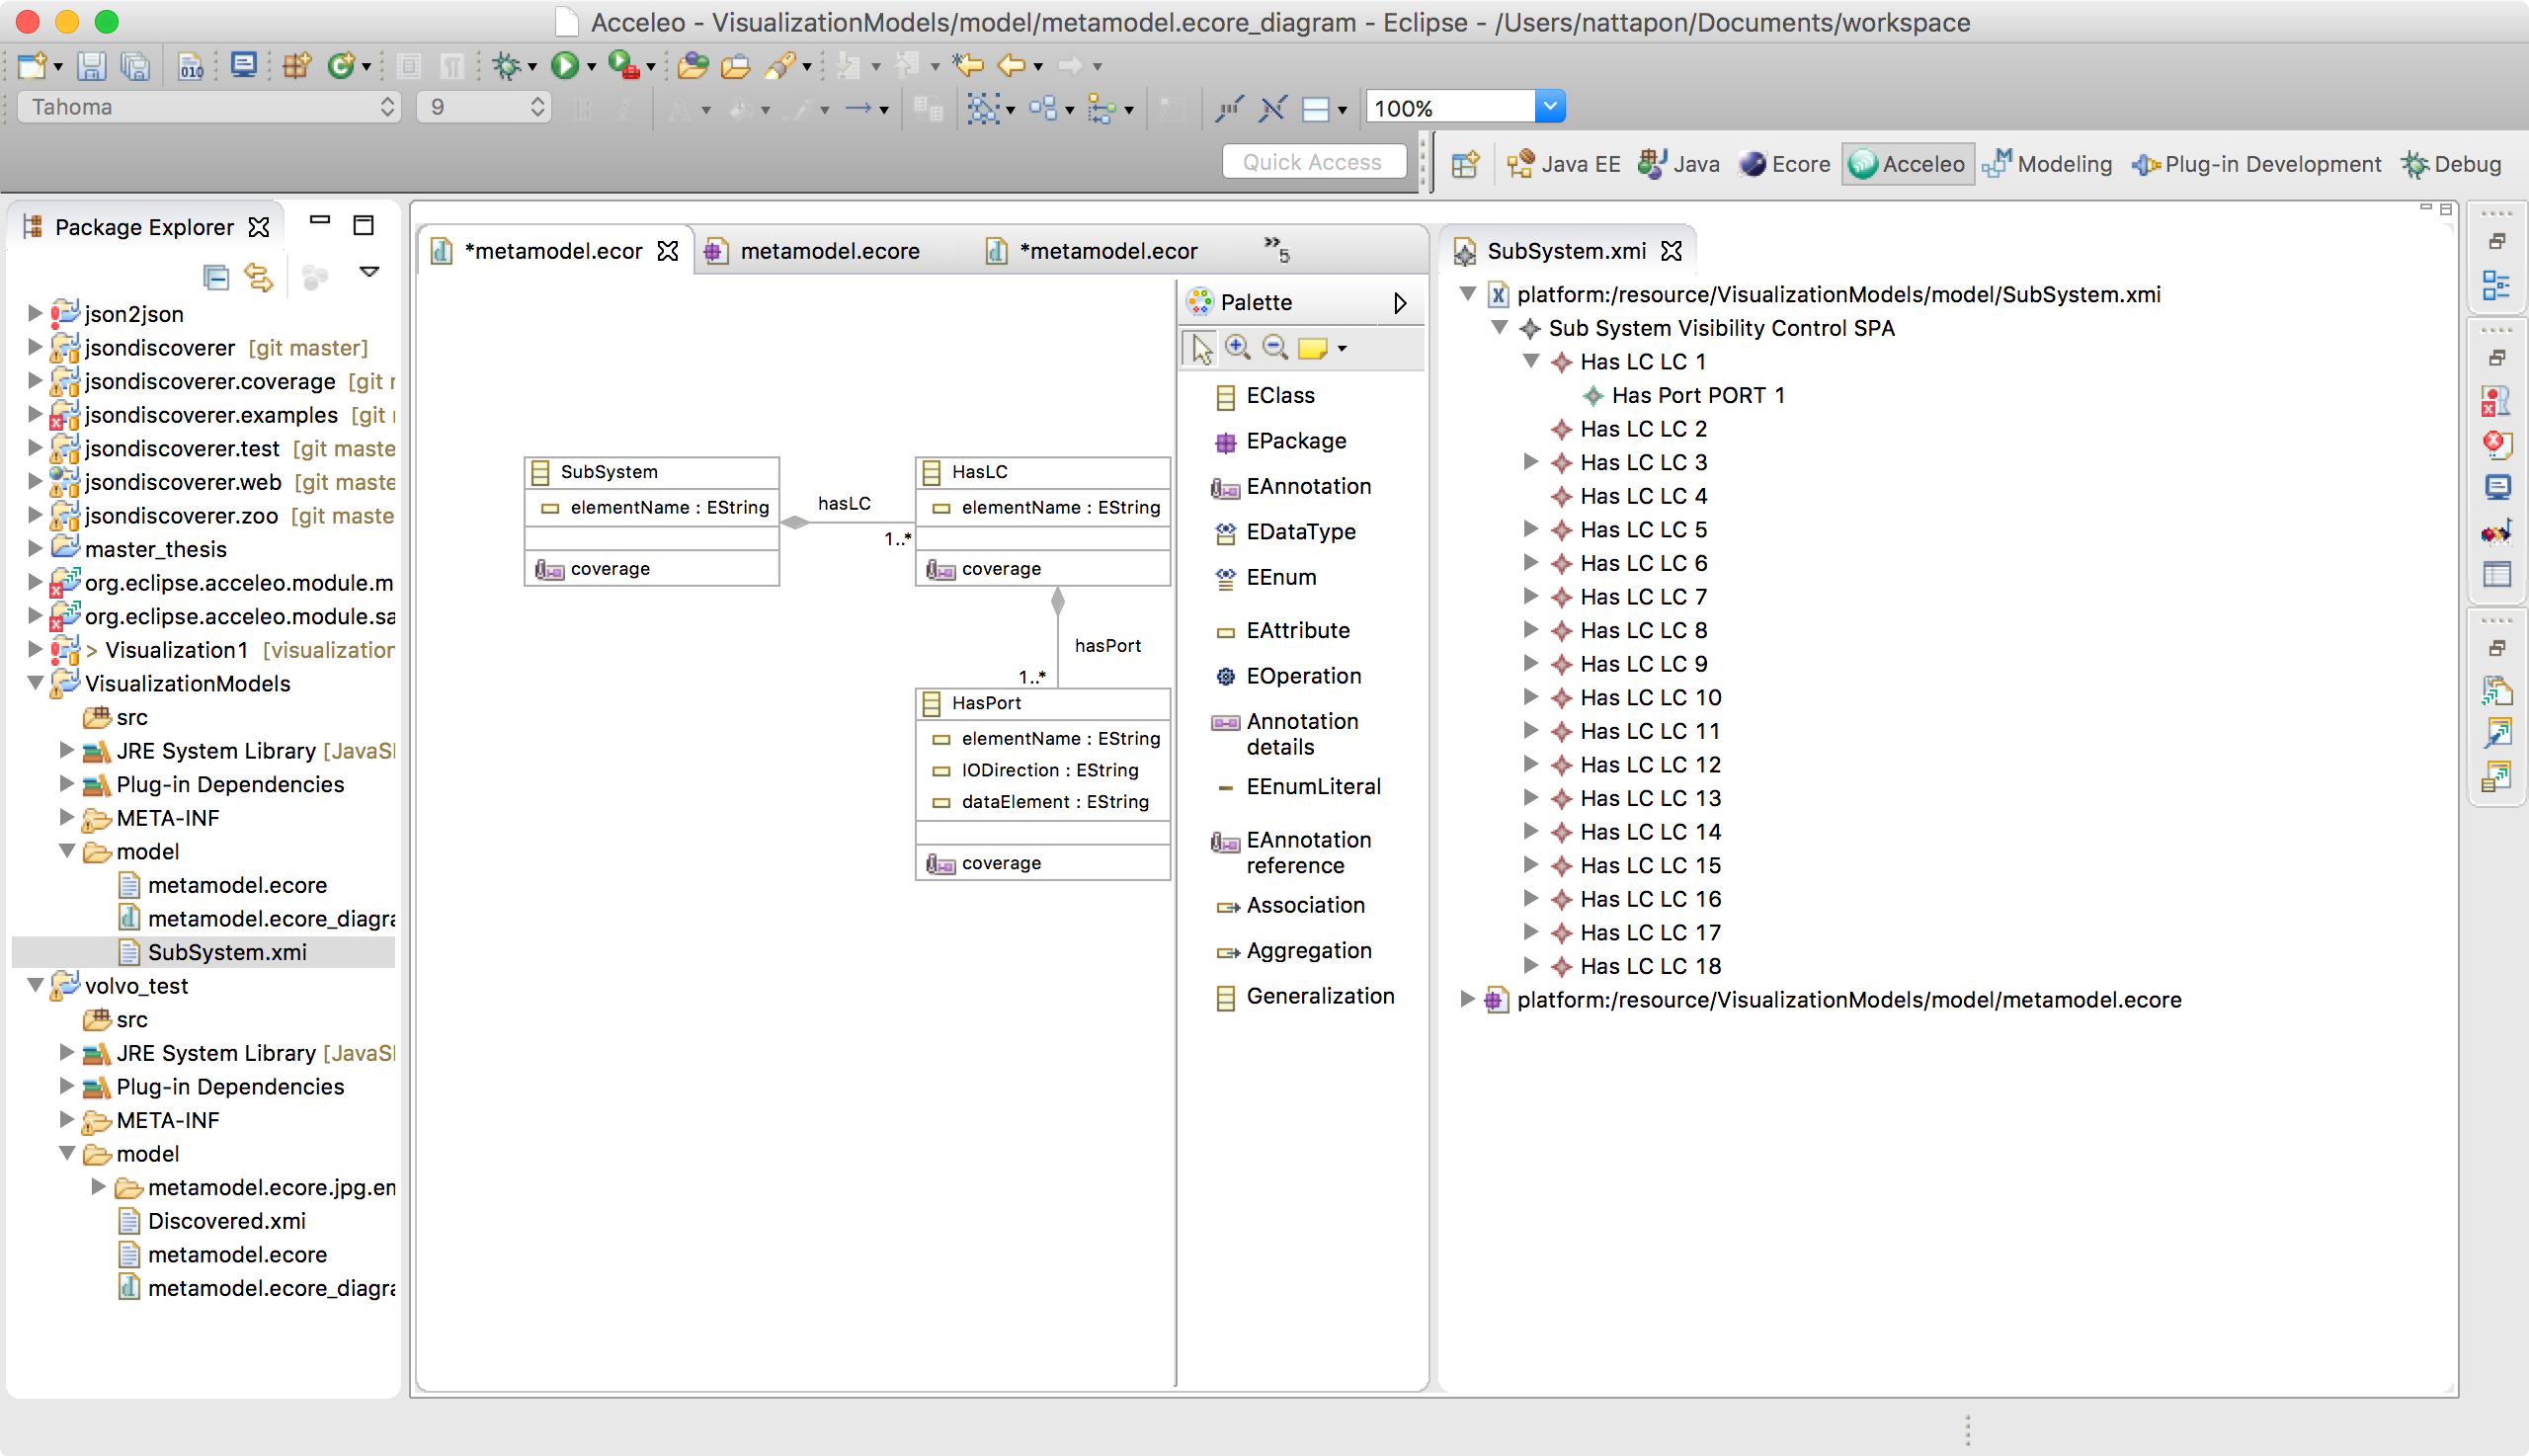
\includegraphics[width=0.95\linewidth]{figure/misc/screenshot_ecore_editor.png}
\caption{A screenshot of Graphical Ecore Editor in Eclipse}
\label{fig:screenshot_ecore_editor}
\end{figure}

An alternative way of creating a meta-model and a model instance is to use \textit{JSON discoverer}\footnote{\url{http://som-research.uoc.edu/tools/jsonDiscoverer/}}. JSON discoverer is an open-source project developed by Javier Luis Cánovas Izquierdo and Jordi Cabot. It provides a feature that automatically discovers the implicit schema (meta-model) and a data model (model instance) of a JavaScript Object Notation (JSON) document.\\ 

In our case, choosing JSON discoverer tool is a good practice since data in the Database can be extracted in JSON format. To create a meta-model and the model instance, we simply imported the JSON file as an input to the tool. An explanation of how to do so will be discussed in Chapter~\ref{methodology}.


\subsection{Model transformation}
\label{model_transformation}
Model transformation is another core concept of MDSE as seen in the equation~\ref{eg:mde} proposed by Stachowiak~\cite{Stachowiak}. Model transformation allows the mappings between different models. One example is transforming UML class diagram\footnote{A static structure diagram that represents the structure of a system showing classes, attributes, methods, and the relations among objects.} to Entity-relationship (ER) diagram\footnote{A data model that describes data in business aspect.}. \\


There are two kinds of model transformation, model-to-model (M2M) and model-to-text (M2T) transformation. M2M transformation takes in a source model as the input and the output is named a target model. The result of M2T transformation is just the strings. The model transformation can be done by using  template-based approach or visitor-based approach~\cite{Czarnecki}. In this work, we were mostly interested with M2T transformation and we applied template-based approach. A number of template engines are available to do a M2T transformation. The template engines are capable of generating files with texts of different formats depending on how the generator file has been programed. The content of a generated file(s) depends on the meta-model specified and also the model instance of a meta-model, this will be discussed in details in Section~\ref{IM:automated_visualization_prototype}. An example of M2T transformation can be seen in Figure~\ref{fig:brambilla-m2t}. \\

\begin{figure}[H]
\centering
\captionsetup{justification=centering}
\vspace{0cm}% Adjust vertical spacing here
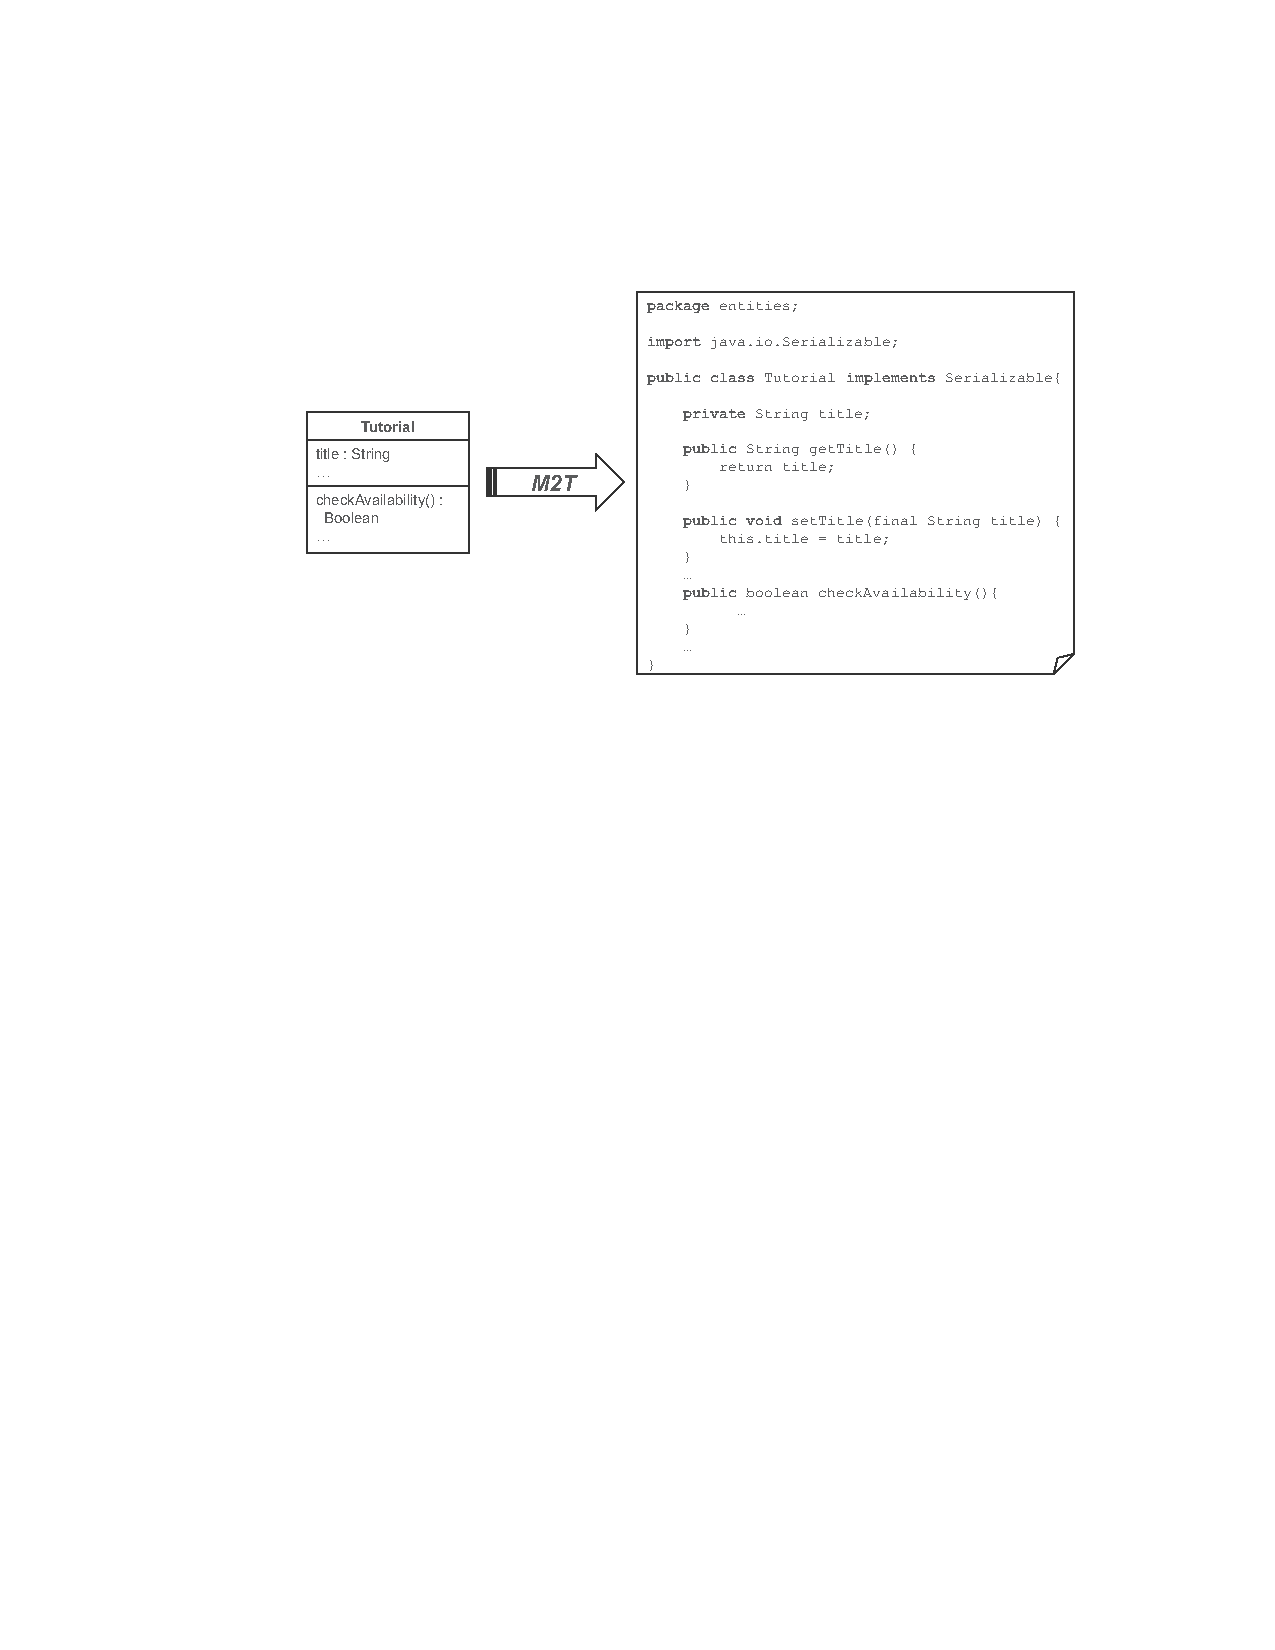
\includegraphics[width=0.8\linewidth]{figure/literatures/brambilla_m2t_example.pdf}
\caption{An example of M2T transformation~\cite{Brambilla}}
\label{fig:brambilla-m2t}
\end{figure}

We used \textit{Acceleo}\footnote{\url{https://eclipse.org/acceleo/}} as the template engine. The structure of an Acceleo template (see Listing~\ref{code:acceleo_template_example}) is composed of module, template, main, and generating files. Module in Line~\ref{line:acceleo_exam_module} is the part where Uniform Resource Identifiers (URIs) of the meta-models instantiating the models that you want to generate code from are parameterized. Template in Line~\ref{line:acceleo_exam_template} is where the name of the template and its parameters are specified. The parameters are declared in the convention \texttt{<name>:<type>}, where \texttt{name} is the parameter name belonging to \texttt{type} which is provided by meta-model. The code in Line~\ref{line:acceleo_exam_main} indicates the entry point of the generation. Line~\ref{line:acceleo_exam_file} is for specifying the name of generated file. The code written after that will be generate textual description. 

\begin{lstlisting}[escapechar=|,caption=An example of Acceleo template, label=code:acceleo_template_example]
[module moduleName('http://www.eclipse.org/emf/2002/Ecore')/]|\label{line:acceleo_exam_module}|
[template public genMyTemplate(aParam: EClass)]|\label{line:acceleo_exam_template}|
[comment @main/]|\label{line:acceleo_exam_main}|
[file ('filename.txt', false, 'UTF-8')]|\label{line:acceleo_exam_file}|
....
[/template]
\end{lstlisting}


\section{Graphical notation of textual description}
The output from M2T transformation is textual description. It is used for generating visualization based on a model instance, which conforms to its meta-model. To create a visualization of the electrical architectures, several tools such as PlantUML\footnote{\url{http://plantuml.com/}} and Umple\footnote{\url{http://cruise.eecs.uottawa.ca/umple/}} can be used. We chose PlantUML as a graph visualization tool. PlantUML is an open-source project developed by Arnaud Roques. The tool allows users to create UML diagrams from textual description written in its DSL. The language of PlantUML is well-formed and human-readable code from which the diagrams are rendered.

\begin{lstlisting}[caption=An example of textual description of a class diagram, label=code:plantuml_class]
@startuml

class Accommodation {
  +Int Floor
  +Int Wall
  +Int Ceiling
  +Int Door
  +Int Window
}

class Apartment
class House

Accommodation <|-left- Apartment: Inheritance
Accommodation <|-right- House: Inheritance

@enduml
\end{lstlisting}

\begin{figure}[H]
\centering
\captionsetup{justification=centering}
\vspace{0cm}% Adjust vertical spacing here
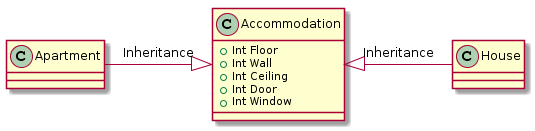
\includegraphics[width=0.8\linewidth]{figure/misc/plantuml_class.png}
\caption{UML class diagram rendered from the textual description in Listing~\ref{code:plantuml_class}}
\label{fig:plantuml_class}
\end{figure}

Different types of UML diagrams such as class diagrams can be generated. Figure~\ref{fig:plantuml_class} shows the UML class diagram rendered from the code in Listing~\ref{code:plantuml_class}.\\

UML component diagrams can also be created from the textual description by using some specific syntax. Table~\ref{table:plantuml_component_syntax} shows the examples of how to use PlantUML syntax. The use of them will be explained in Chapter~\ref{implementation}. 

%\begin{table}[H]
%\centering
%\renewcommand{\arraystretch}{1.5}% Spread rows out...
\begin{longtable}{>{\centering}m{1.8in} >{\centering}m{2in} >{\centering\arraybackslash}m{1.5in}}
\toprule
\textbf{Description} & \textbf{PlantUML syntax} & \textbf{Representation} \\
\midrule
Package & \texttt{package Package} & 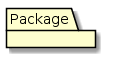
\includegraphics[width=0.5\linewidth]{figure/plantuml_example/package.png} \\ \hline
Component & \texttt{[component]} & 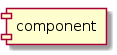
\includegraphics[width=0.5\linewidth]{figure/plantuml_example/component.png} \\ \hline
Components, ports, \\and connection &  \texttt{[c1] \#-\# [c2]} & 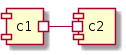
\includegraphics[width=0.6\linewidth]{figure/plantuml_example/port.png}\\ \hline
Components, and ports with required/provided interfaces & \texttt{[c1] \#-(0-\# [c2]} & 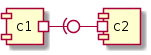
\includegraphics[width=0.8\linewidth]{figure/plantuml_example/port_type.png}\\ \hline
Rectangle & \texttt{rectangle Rectangle} & 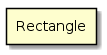
\includegraphics[width=0.5\linewidth]{figure/plantuml_example/rectangle.png}\\ \hline
Component, required interface, and rectangle & \texttt{rectangle Rectangle} \\ \texttt{[c1] -( Rectangle} & 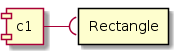
\includegraphics[width=0.8\linewidth]{figure/plantuml_example/component_rectangle.png}\\
\bottomrule
\caption{Some useful syntax for UML component diagrams}
\label{table:plantuml_component_syntax}
\end{longtable}
%\end{table}

With the combination and modification of the syntax, visualizing electrical architectures is possible.
%%%%%%